\chapter{从定性到定量} % Introduction chapter suppressed from the table of contents

当团队已经掌握好迭代回顾根因分析后,便可以尝试利用蒙特卡洛(Monte
Carlo)预测模型做定量分析。

下面介绍如何利用蒙特卡洛预测模型帮助团队分析迭代缺陷数据,并预测下个迭代(改进后)的过程缺陷范围,把缺陷管理从以前定性,提升到量化管理。

\hypertarget{ux4f7fux7528ux7f3aux9677ux6392ux9664ux7387ux914dux5408ux8499ux5730ux5361ux7f57ux9884ux6d4bux6a21ux578bux505aux5b9aux91cfux5206ux6790}{%
\subsection{使用缺陷排除率,配合蒙特卡洛预测模型做定量分析}\label{ux4f7fux7528ux7f3aux9677ux6392ux9664ux7387ux914dux5408ux8499ux5730ux5361ux7f57ux9884ux6d4bux6a21ux578bux505aux5b9aux91cfux5206ux6790}}

\begin{enumerate}
\tightlist
\item
  依据客户需求和公司基线与目标,设定下次迭代量化目标。例如希望最终遗漏到验收发现的缺陷数降多少?
\item
  并设定过程目标缺陷数,从而预测能否达到最终目标,缺陷越能在前面过程(如需求/设计评审)发现并解决缺陷,后面过程里发现的缺陷会减少
  (假定每个过程引入的缺陷数没有重大改变)
\end{enumerate}

如果要最终质量好,缺陷排除率就要高。但计算缺陷排除率,必须要等到整个开发完成才可以计算,我们可以建立预测模型,模拟这个过程:\\
需求会引入缺陷,然后需求评审排除缺陷等等。把各引入缺陷数,排除率输进蒙特卡洛预测模型,然后使用它估计每个阶段的缺陷数量范围。

参照前面提过的缺陷排除率(DRE) 计算公式:

%Ma3_10.png

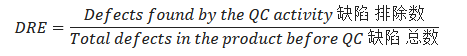
\includegraphics[width=10cm]{Ma3_10.png}

%\href{文件:1113correctEgScreenshot_2021-11-13_212414.png}{400px}

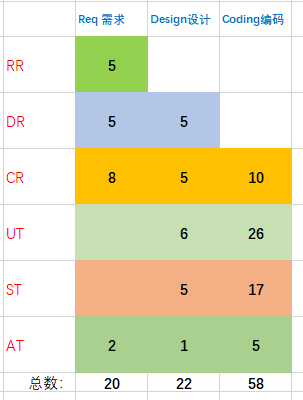
\includegraphics[width=10cm]{1113correctEgScreenshot_2021-11-13_212414.png}

%\href{文件:1113corrDreScreenshot_2021-11-13_212509.png}{600px}

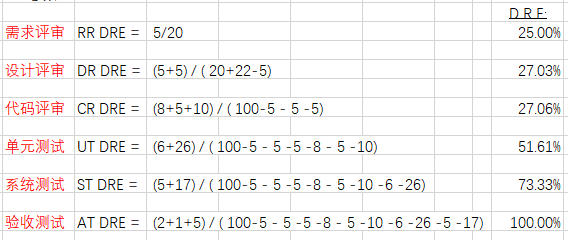
\includegraphics[width=10cm]{1113corrDreScreenshot_2021-11-13_212509.png}

得出下面Figure7.2,缺陷分布是中间最高头尾低,右面与左面不同,有条长尾巴,类似估算软件开发项目工作量的
Rayleigh 曲线。

%\href{文件:jalote_emm_7.2.png}{500px}

\includegraphics[width=10cm]{jalote_emm_72.png}

模型假定每个阶段的缺陷排除率都比较稳定,在某个范围之内,不同阶段引入的缺陷也在一定范围之内。

\hypertarget{ux600eux6837ux5f00ux59cb}{%
\subsection{怎样开始}\label{ux600eux6837ux5f00ux59cb}}

培训能让团队能先了解利用模拟工具量化管理的原理,也让团队为收集迭代数据做准备,所以建议先做模拟互动培训。下面是一天互动培训的时间安排:(上午是做上一章迭代回顾的互动练习,下午是使用蒙特卡洛预测模型预测下迭代的互动练习。)

\href{文件:712trainingAgendaScreenshot_2022-07-12_125030.jpg}{500px}

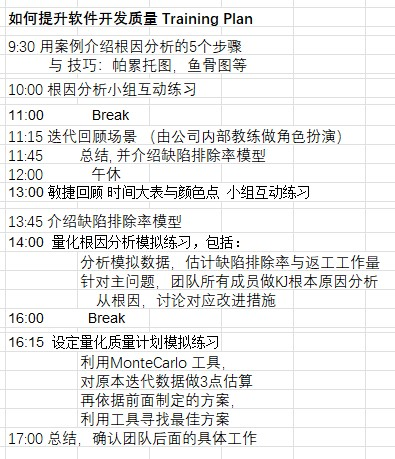
\includegraphics[width=10cm]{712trainingAgendaScreenshot_2022-07-12_125030.jpg}

\hypertarget{ux65f6ux95f4ux5b89ux6392}{%
\subsubsection{时间安排}\label{ux65f6ux95f4ux5b89ux6392}}

如果是首次根本原因分析培训,建议先在培训当天早上做以下根因分析小组互动练习,让大家先熟悉根因分析的重点:

\begin{itemize}
\tightlist
\item
  提供一对模拟数据,要求团队利用帕累托图加鱼骨图分析,找出根本原因与改进措施
\item
  目的:让团队先感受如何基于数据,找出根本原因
\end{itemize}

\hypertarget{ux57f9ux8badux5bf9ux8c61}{%
\subsubsection{培训对象}\label{ux57f9ux8badux5bf9ux8c61}}

\begin{itemize}
\tightlist
\item
  后面会参与试点的项目组,培训后可以把学过的在项目里实践
\item
  所有团队角色都参加
\end{itemize}

\hypertarget{ux51c6ux5907ux6570ux636eux8ba9ux56e2ux961fux6a21ux62df}{%
\subsubsection{准备数据,让团队模拟}\label{ux51c6ux5907ux6570ux636eux8ba9ux56e2ux961fux6a21ux62df}}

要做量化根本原因分析就必须要有数据,所以内部教练须要预先准备下面缺陷与返工工作量数据,类似一轮冲刺后的场景:

\begin{enumerate}
\tightlist
\item
  系统测试缺陷数据,建议从缺陷管理工具里抽取,40 - 60 项
\item
  开发个人系统测试BUG返工工时统计表:那个BUG号 / 总修复工时 / 备注
\item
  开发个人开发期间用于修复评审/单元测试返工工时统计表:那个模块 /
  总修复工时 / 备注
\end{enumerate}

\begin{itemize}
\tightlist
\item
  打印以上的数据表,发给团队做练习时参考
\end{itemize}

例如,互动练习时,要学员利用开发人员工时表
(模拟他们迭代中用于改缺陷的工时,与评审缺陷数,与开发和修正代码的工时):

%\href{文件:缺陷表4.jpg}{500px}

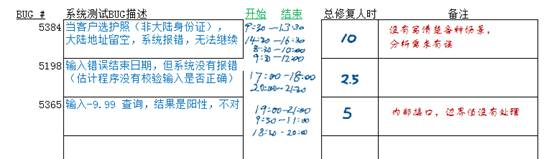
\includegraphics[width=10cm]{缺陷表41.jpg}

%\href{文件:微信截图_20211228095232.png}{500px}

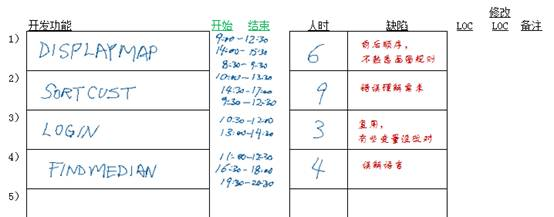
\includegraphics[width=10cm]{缺陷表51.jpg}

\hypertarget{ux51c6ux5907ux5de5ux5177}{%
\subsubsection{准备工具}\label{ux51c6ux5907ux5de5ux5177}}

\begin{itemize}
\tightlist
\item
  分2-4组,6-8人一组,,需要有一个大而光亮的会议室,
  方便小组互动,大白板和架子,各种颜色的水笔,墙壁可以贴上小组的白纸
\item
  教练提供有MonteCarlo工具的笔记本电脑
\end{itemize}

\hypertarget{ux67d0ux516cux53f8ux7ecfux8fc7ux57f9ux8badux540eux7b2cux4e00ux8f6eux56deux987eux4f8bux5b50}{%
\subsection{某公司经过培训后第一轮回顾例子}\label{ux67d0ux516cux53f8ux7ecfux8fc7ux57f9ux8badux540eux7b2cux4e00ux8f6eux56deux987eux4f8bux5b50}}

\begin{itemize}
\tightlist
\item
  团队分析迭代缺陷数据,缺陷是源自需求/设计/编码,得出以下分布表:
\end{itemize}

%\url{文件:微信截图_20220316093044.jpg}


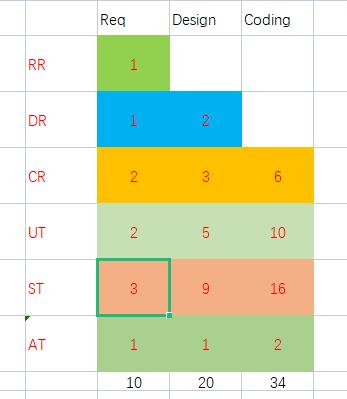
\includegraphics[width=10cm]{微信截图_20220316093044.jpg}

\begin{itemize}
\tightlist
\item
  按DRE公式,计算出各个过程的缺陷排除率
\end{itemize}

%\href{文件:2DreEstimateScreenshot_2021-12-01_212049.png}{400px}\\

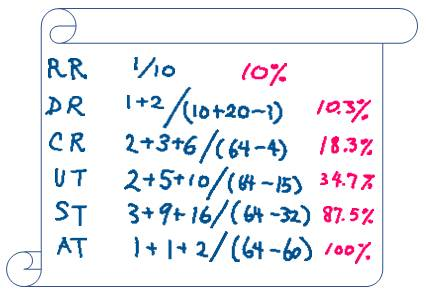
\includegraphics[width=10cm]{2DreEstimateScreenshot_2021-12-01_2120491.jpg}

\begin{itemize}
\tightlist
\item
  从团队工时表估算各过程的缺陷返工工作量
\end{itemize}

%\href{文件:4reworkByPhaseScreenshot_2021-12-01_214838.png}{450px}

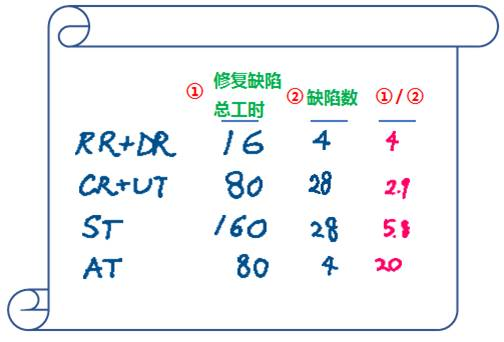
\includegraphics[width=10cm]{4reworkByPhaseScreenshot_2021-12-01_2148381.jpg}

\begin{itemize}
\tightlist
\item
  把缺陷排除率与返工工作量输入预测模型,得出每个过程的缺陷范围与质量成本,也验证了是系统测试缺陷率最高
\end{itemize}

%\href{文件:2AxtalBallPredictScreenshot_2021-12-01_212455.png}{400px}\\

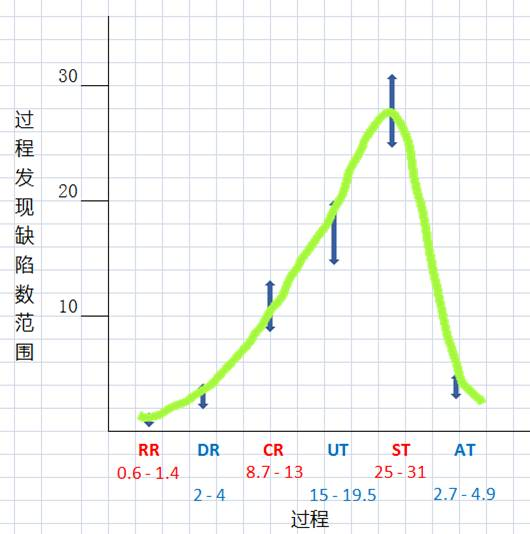
\includegraphics[width=10cm]{2AxtalBallPredictScreenshot_2021-12-01_2124551.jpg}

\begin{itemize}
\tightlist
\item
  团队针对评审排除率低(如需求/设计评审)、利用新的技术和工具,例如用原型法和新评估方法,能提高需求与设计的缺陷排除率。把新方法的预估排除率加进预测模型,然后使用模型比较各种方法,寻找那个搭配的返工工作量最低,模型能预测使用新方法后的各个过程缺陷范围与质量成本。
\end{itemize}

如果没有预测模型,我们只能主观估计百分比会降低,但有了预测模型,我们确实可以尝试改变参数,看能否估计缺陷分布的变化,也帮我们验证这假定是否可行。最终我们验证了确实这个百分比是可行。如果没有预测模型便难以做到。

例如,延续前面例子,下面看看团队如何基于练习2的数据,加入新方法/新参数,利用模型预估下一轮缺陷分布:

%\url{文件:微信截图_20211207132712.png}

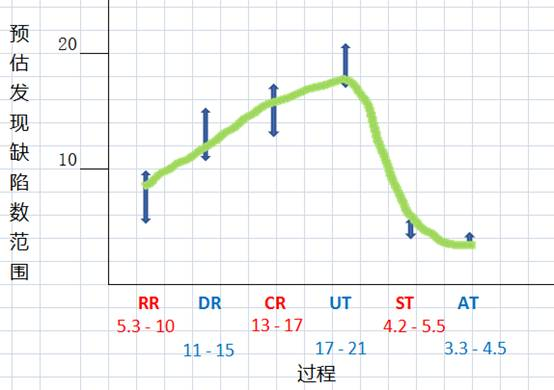
\includegraphics[width=10cm]{微信截图_202112071327121.jpg}

可看到大部分缺陷都前移,系统测试缺陷下降。

\hypertarget{ux603bux7ed3}{%
\subsection{总结}\label{ux603bux7ed3}}

当数据不是单点而是分布时,蒙特卡罗预测模型可以帮我们更好处理数据。针对如何可以把发现缺陷前移的例子里,模型可以从每个过程的分布预估总返工工作量成本分布,也可以比较不同的搭配,自动挑选哪个搭配的质量成本最低。要做好回顾分析,最困难不是数据分析,而是怎么收集到真实的数据。所以必须在培训里,让学员知道为什么要收集数据,为迭代收集数据做好准备。

整个迭代回顾过程:要做好迭代,必须所有干系人都参与,并要花大概3、4个小时的精力分析、讨论改进行动,所以必须以二八原则挑选最容易出效果的方案,才容易得到高层的支持,也需要培训团队各种分析技巧和原则。

如果希望干系人有执行改进行动的动力,必须要他们在回顾时全心投入参与讨论,一起找根本原因和解决方案。所以培训时,不仅仅是教分析的技巧,更需要让他们可以放心发表意见。如果把培训设计成互动游戏,可避免迭代回顾时,项目经理一言堂的现象。

分析的方法和可以改进的方向很多,这几个章节主要以一些实例带出每一个步骤的重点。大家掌握了这些节奏之后,就可以融会贯通,持续进行根本原因分析,形成不断优化的良性循环。目标是提升产品的质量,而不是习惯于当前的缺陷水平,缺乏改进动力。要做好根本原因分析,收集到正确有用的数据非常关键。在VI部分我们会探索度量与分析的重点。

\hypertarget{ux9644ux4ef6}{%
\section{附件}\label{ux9644ux4ef6}}

\hypertarget{ux6c34ux6676ux7403ux8499ux5730ux5361ux7f57ux9884ux6d4bux6a21ux578b}{%
\subsection{蒙特卡洛预测模型}\label{ux6c34ux6676ux7403ux8499ux5730ux5361ux7f57ux9884ux6d4bux6a21ux578b}}

\begin{itemize}
\tightlist
\item
  按每个过程的统计数据,估计对应缺陷排除百分比的上下限与均值,工作量也类似。例如,从公司基线,代码走查的缺陷排除率是55\%左右;评审总工作量(不包含修正缺陷)大概为20人时。如果开始时没有充足的项目数据,可以先依据行业基线:如代码正式审查应能排除85\%,但平均人时会增加到35人时
  (也是不包含修正缺陷)。得出下图:
\end{itemize}

%\href{文件:微信截图_20211027011246.png}{450px}

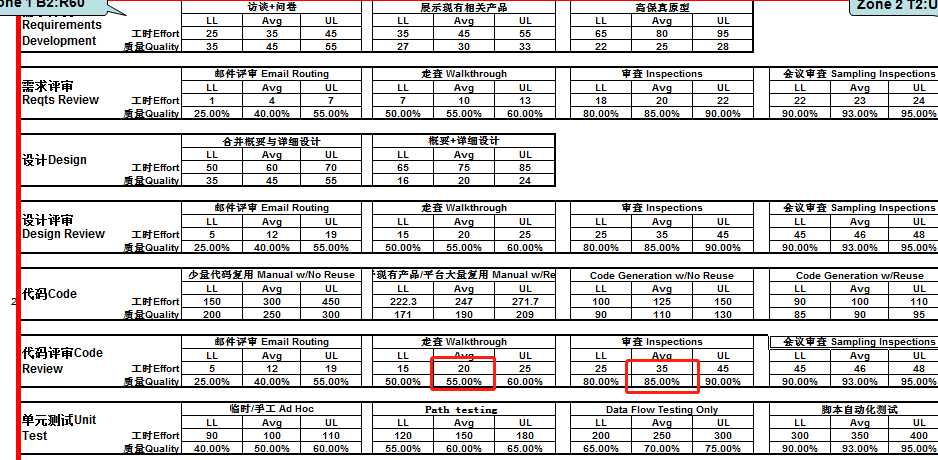
\includegraphics[width=10cm]{微信截图_20211027011246.png}

\begin{itemize}
\tightlist
\item
  模型会自动按输入的最大最小值计算标准差,变成分布(如:正态(normal)分布、三角形(triangular)分布),水晶球模型会依据黄格里的数字选取对应的分布,
\end{itemize}

%\href{文件:微信截图_20211027011403.png}{450px}

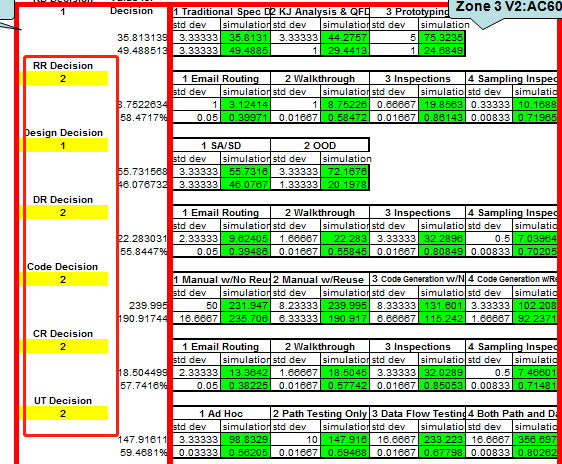
\includegraphics[width=10cm]{微信截图_20211027011403.png}

\begin{itemize}
\tightlist
\item
  取对应的分布,依据项目历史数据统计,估算各个过程缺陷的返工工作量与成本。例如:修复一个系统测试发现的缺陷,平均要用6000元,最高7500,最低5000。如果缺陷导致的如果是工时那行,填上对应工种的平均人时总成本。水晶球模型就会依据我们输入的范围估算单位成本的分布,放在绿格里。
\end{itemize}

%\href{文件:微信截图_20211027012006.png}{450px}

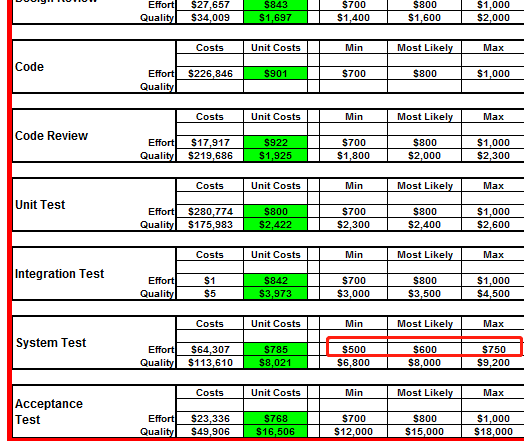
\includegraphics[width=10cm]{微信截图_20211027012006.png}

\begin{itemize}
\tightlist
\item
  如果从需求到验收测试,每一个过程的成本数都是单一值; 我们可以简单用 XLS
  把数加起来得出总数。但如果每个过程的成本数都是一个分布,例如三角形分布,
\end{itemize}

必须要使用蒙特卡洛方法才可以把每个过程''加''起来。

\begin{itemize}
\tightlist
\item
  水晶球可以帮我们估计质量成本的分布,例如我们需求评审用审查(2),设计评审用走查(2)
  ,代码评审也用走查(2),单元测试是手工(1),系统测试估计走3轮(2),验收测试预计走3轮(2),水晶球就会依据我们刚刚输入的分布用蒙特卡洛预测模型预估质量成本的分布。
\end{itemize}

%\href{文件:HmttDistScreenshot_2021-10-08_165836.png}{450px}

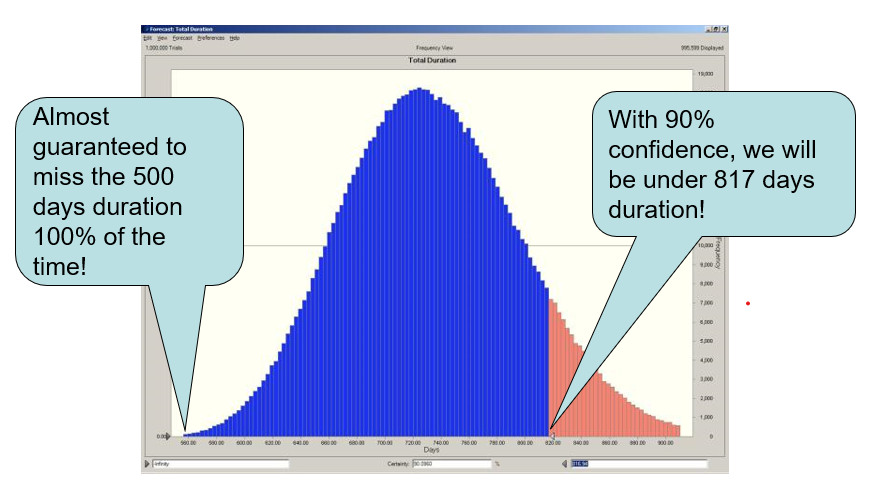
\includegraphics[width=10cm]{HmttDistScreenshot_2021-10-08_165836.png}

\begin{itemize}
\tightlist
\item
  比较各种不同的配搭,选出质量成本最低是哪个配搭组合,帮助项目组在策划时选择使用什么方法,得出最佳效果。
\end{itemize}

下图显示一直水晶球优化的过程,和最终的最``佳''配搭:\\
%\href{文件:HmttOptScreenshot_2021-10-08_165653.png}{450px}

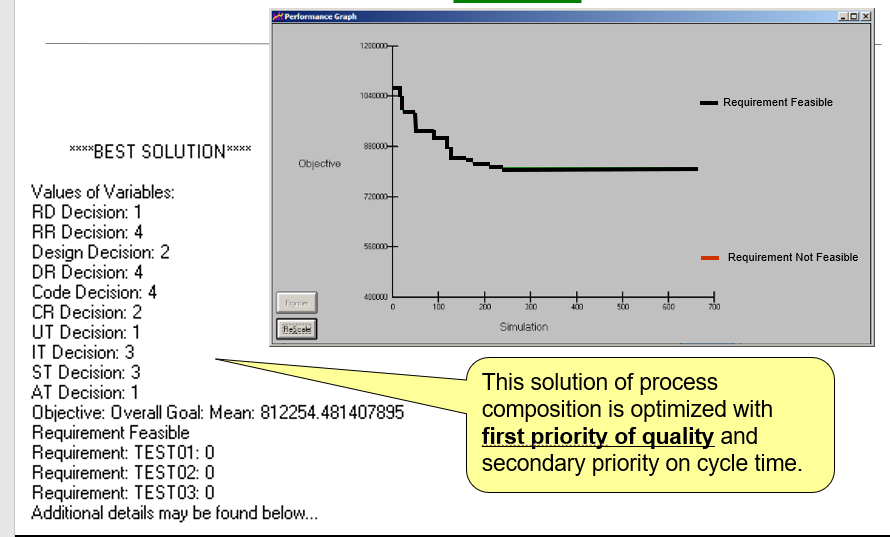
\includegraphics[width=10cm]{HmttOptScreenshot_2021-10-08_165653.png}

在需求评审,设计评审,代码评审,单元测试,系统测试,验收测试都有两种选择时,跑优化,95\%的置信区间
得出 Overrall goal (Quality + Effort) = 1,476,773美元

%\href{文件:微信截图_20211103023018.png}{600px}

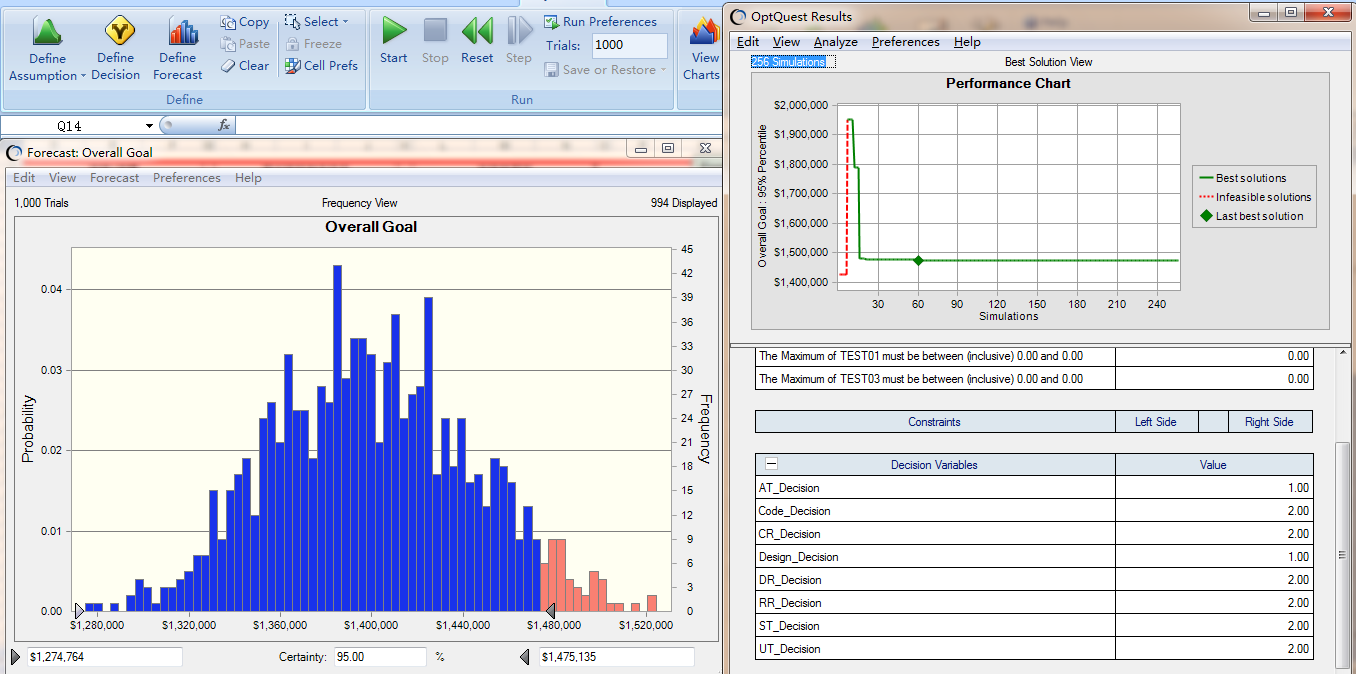
\includegraphics[width=10cm]{微信截图_20211103023018.png}



